\documentclass[11.5pt]{article}

\usepackage{fontenc}
\usepackage{lmodern}
\usepackage{gensymb}
\usepackage[english]{babel}
\usepackage{fancyhdr}
\usepackage[shortlabels]{enumitem}
\usepackage{authblk}
\usepackage[utf8]{inputenc}
\usepackage{amsmath}
\usepackage{amsfonts}
\usepackage{amssymb}
\usepackage{natbib}
\usepackage{graphicx}
\usepackage{mathtools}
\usepackage{lipsum}
\usepackage{xparse}
\newcommand\hr{\par\vspace{-.5\ht\strutbox}\noindent\hrulefill\par}
\graphicspath{ {./images/} }
\renewcommand{\thesection}{\Roman{section}}
% \renewcommand{\thesubsection}{\thesection.\Roman{subsection}}
\NewDocumentCommand{\set}{o m}{%
  % <code>
  \IfNoValueTF{#1}
    {\{#2\}}
    {\{#1 \mid #2\}}%
  % <code>
}
\usepackage{hyperref}
\hypersetup{
    colorlinks=true,
    linkcolor=blue,
    filecolor=magenta,      
    urlcolor=cyan,
}
\urlstyle{same}
\newcommand\norm[1]{\left\lVert#1\right\rVert}
\DeclareMathOperator*{\argmax}{arg\,max}
\DeclareMathOperator*{\argmin}{arg\,min}
\usepackage{indentfirst}
\usepackage{geometry}
 \geometry{
 a4paper,
 left=15mm,
 top=8mm,
 right=15mm
 }
\usepackage{tabularx}
\usepackage[english]{babel}
\usepackage{multicol}
\usepackage{pdfpages}


\title{\textbf{MACHINE LEARNING LAB PROJECT}\hr \textit{\textbf{Fake News Detection: A Machine Learning Approach}}\hr}

\author[1]{154446$^*$ -- Fopa Yuffon Amadou Olabi}
\author[2]{160041082 -- Mohamed Moctar}
\author[3]{160041083 -- Tani Barakat Shalanyuy}
\author[4]{160041085 -- Mikayilou Namba}
\author[5]{160041087 -- Aly Abdel Kader Gelany}
\author[6]{160041006 -- Muhammed Barry}
\affil[1]{$^{,2,3,4,5,6}$ Department of Computer Science and Engineering, Islamic University of Technology\hr}

\date{$16^{th}$ September 2020.}

\begin{document}

\maketitle
\begin{multicols}{2}

\paragraph{Abstract---}
Fake News and Scams started since the web time frame. The fake news design started basically to dupe per-clients, increase readership and is oftentimes used as a strategies for mental battling. Advances in development and the spread of news through different sorts of media, without truly checking the real factors, have extended the spread of fake news today. The essential purpose behind this endeavor is to devised a classifier which can isolate fake news from the certifiable news.
\newline
We propose in this research project, a fake news detection model that uses a Text Vectorizer and machine learning techniques to tackle the problem.
Experimental evaluation yields the best performance using Term Frequency-Inverted Document Frequency (TF-IDF) as feature extraction technique, and Passive Aggressive Classifier as a classifier, with an accuracy of more than \textbf{97\%}. 

\paragraph{Keywords---}
Fake News, Real News, Machine Learning Techniques, Text classification, TF-IDF Vectorizer, Term Frequency (TF), Inverse Document Frequency (IDF), Passive Aggressive Classifier (PAC), Python.

\section{Introduction}
\paragraph{}
The effects of fake news have increased exponentially in the recent past and something must be done to prevent this from continuing in the future. The dangerous effects of fake news, as previously defined, are made clear by events such as in which a man attacked a pizzeria due to a widespread fake news article. This story along with analysis provide evidence that humans are not very good at detecting fake news, possibly not better than chance. As such, the question remains whether machines can do a better job. A machine can solve the fake news problem using supervised learning that extracts features of the language and content only within the source in question, without utilizing any fact checker or knowledge base.
\newline
Do you trust all the news you hear from social media? All news is not real, right?
So how will you detect the fake news? The answer is Python.
\newline
By practicing such an advanced python project of detecting fake news, we will easily make a difference between real and fake news. Before moving ahead in this advanced Python project, we have to be aware of related terms of fake news like the TF-IDF Vectorizer, and the Passive Aggressive Classifier.
\newline
This project will work you through the necessary steps and techniques used to implement such an analysis.
\begin{center}
    \centering
    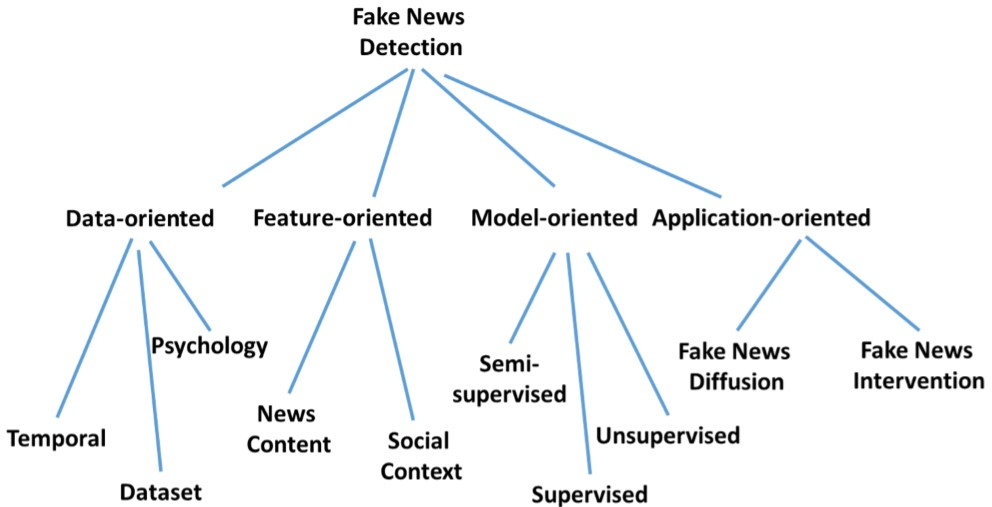
\includegraphics[width=8.8cm]{Future directions and open issues for fake news detection on social media.jpg}
    \caption{\underline{Fig.\ref{fig:project_tree}:} Future directions and open issues for fake news detection on social media}
    \label{fig:project_tree}
\end{center}

\subsection{Problem Statement}
\paragraph{}
This project proposes the question of whether it is possible to detect fake news through machine learning models. Specifically, the aim of this project is to determine the ideal model that is efficient in predicting fake news while also limiting the cost of memory and storage for computation. ”Fake news” has been a very recent and prevalent problem within recent years.

\subsection{Detail of your problem application area/domain}
\paragraph{Fake news}
spreads like a wildfire and this is a big issue in this era. We can learn how to distinguish fake news from a real one. We will be using supervised learning approach to implement the model.

\paragraph{}
As a consequence of the increase in cases of fake news in recent years, efforts have been made to crackdown on the spread of misinformation throughout social media platforms. All popular social media platforms (Facebook, Twitter, Spotify, and YouTube) have permanently banned Alex Jones from using their networks \citep{alexjones2018banned} following the events of ”Pizza Gate” \citep{pizzagate} in addition to multiple questionable accusations made by Jones, including an accusation made by Jones claiming that the Sandy Hook shooting was ”faked”.

\paragraph{}
Despite efforts of many social media websites and governments cracking down on fake news, many young people today generally are not able to tell the difference between fake news and real news. According to a Stanford study it found that many students have a very strong inability in discerning between fake news. In the study, high school students were given two posts announcing the candidacy of Donald Trump’s presidential Campaign. One post was given by an actual Fox News account another one posted by an account that ”looked” like it was from Fox News. 25\% of the could not tell the difference between real and fake news sources. With over 30\% of students favoring that the fake news account was more trustworthy.

\paragraph{}
Indeed, some politically charged or bogus articles that would be esteemed false frequently have more perspectives and offers via web-based media destinations than real news stories towards the most recent three months of the political race. As per an examination by Buzz-channel, posts and stories composed from the best twenty most noteworthy performing trick locales and hyper-hardliners had over 8.7 million offers, "responses" and remarks contrasted with the main twenty most noteworthy performing significant news associations had about 7.4 million offers, "responses" and remarks via online media destinations.

\paragraph{}
The research problem was initially defined through the following use cases: In light of a single event/story, the framework would decide whether certain sources or articles are regarded to be fake news dependent on a given likelihood. Through the sources analyzed the machine learning agent would assign an level of bias and factuality of these articles by comparing them to each other and assign scores of the sources bias and factuality.

\paragraph{}
A sort of sensationalist reporting, counterfeit news exemplifies bits of news that might be scams and is commonly spread through web-based media and other online media. This is regularly done to further or force certain thoughts and is frequently accomplished with political plans. Such news things may contain bogus and additionally overstated cases and may wind up being viral by calculations, and clients may wind up in a channel bubble.

\subsection{Challenges and Motivation}
\paragraph{Motivation---}
The motivation for research on this topic was that this is a relatively new area of research with many opinions but not many concrete solutions. Many implementations focus primarily on the host of the article, but even articles hosted on otherwise trustworthy websites can be classified as fake news. The primary motivation of this project was to bring awareness,propose a solution,and work towards minimizing the effects of fake news.

\paragraph{Challenges---}
Throughout the project and its analysis study, we faced some challenges such as:
\begin{itemize}
    \item \textbf{Data Collection}: While collecting the data, we faced an issue with the relation of topics among news feeds. This is due to the variety of categorized topics covered by most informative platforms. 
    \item \textbf{Data Analysis and Interpretation}:
    After collecting these data, we spend a lot of time in analyzing from a feature-based perspective.
    \item \textbf{Data Preprocessing Methodology}:
    After proper analysis and interpretation, we need to prepare and sanitize the data for it to be suitable for more insights on the learning process. 
    \item \textbf{Learning Model Selection}
    (Which model suits well the given problem.)
    \item \textbf{Update the Model for better Accuracy}:
    Here we try to tune the parameters/hyperparameter to obtain a better accuracy from the selected model.
\end{itemize}
\begin{center}
    \centering
    \qquad
    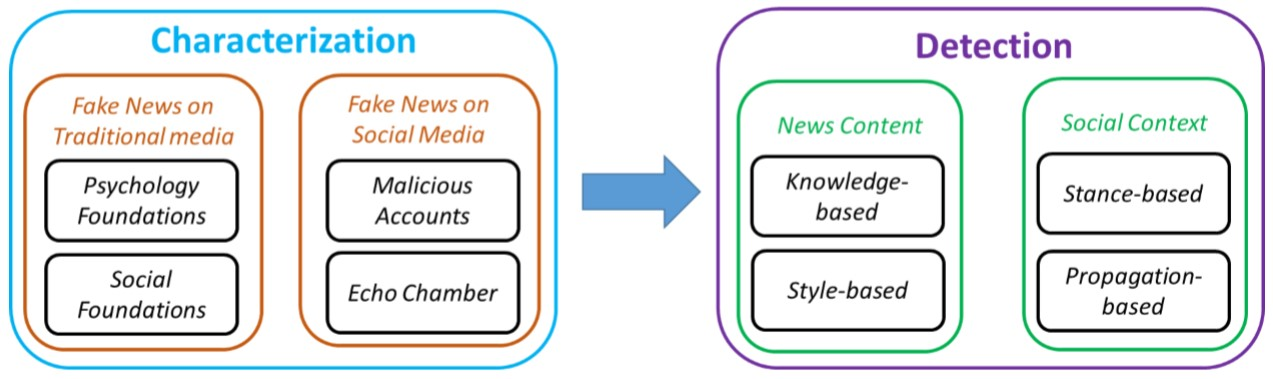
\includegraphics[width=8.8cm]{Fake news on social media -- from characterization to detection.jpg}
    \caption{\underline{Fig.\ref{fig:news_kterization}}: Fake news on social media: from characterization to detection}
    \label{fig:news_kterization}
\end{center}
\subsection{Objectives}
\paragraph{}
The purpose of this paper is to design and implement a machine learning implementation that correctly predicts if a given article would be considered as fake news. The contributions of this paper are as follows
\begin{itemize}
    \item Introduces the topic of fake news and the various machine learning algorithms to build a model to accurately classify a piece of news as REAL or FAKE.
    \item Provides an overview of the history and implications of fake news.
    \item This advanced python project of detecting fake news deals with fake and real news. Using SK-Learn tools, we will a \textbf{TfidfVectorizer} on our dataset.
    \item Then, we initialize a \textbf{PassiveAggressive} Classifier to fit the model, which will result a accuracy score and a confusion matrix that tell us how well our model fares.
    \item Presents a possible solution and lays some ground work in further study in this area.
\end{itemize}

\subsection{Contribution}
\paragraph{}
The project’s contributions are split between five members. 
\textit{Tani Barakat}$^3$ and \textit{Muhammed Barry}$^6$ helped visualize the models’ results through the Sci-Kit and Sea-born libraries. 
\textit{Mohamed Moctar}$^2$ helped with research of the other related works done by external organizations. 
\textit{Aly Abdel Kader G.}$^5$ and \textit{Mikayilou Namba}$^4$ implemented the machine learning models of the project.
\textit{F. Y. Amadou Olabi}$^1$ served as the project lead in conceptualizing the idea and technical writing for the group. And also researched, cleansed and formalized the dataset used for the machine learning techniques and implemented the models. 

\section{Background Study}
\paragraph{}
Several groups and organization have also worked on similar ideas in their own implementations. These works highlight some of the challenges of fake news detection. One implementation by \textit{Katharine Jarmul}, founder of data analysis company \href{run: https://kjamistan.com/}{\textit{Kjamistan}}, uses a Passive Aggressive Classifier to detect fake news \citep{jarmul}.The implementation is a tutorial on using different Bayesian models posted on DataCamp\citep{jarmul},  which offers courses on a variety of data science topics including R and Python.

\paragraph{}
One paper titled \textit{’Exploiting Network Structure to Detect Fake News’}, written by three Stanford University students, also implements a Neural Network for classifying fake news\citep{rao}. Their implementation also takes into account the social context in addition to article-specific features such as the title and content in an article in an attempt to improve prediction accuracy. This is one of the few possible ways to improve prediction accuracy without improving upon the natural language processing.

\paragraph{}
Another paper titled \textit{'Fake News Detection: A Deep Learning Approach'}, implemented three different neural network models to compare with the only difference between them being how they took in the article content and title\citep{thota}.
This indicates that the way one goes about processing text in an article makes a huge difference in the performance of a model. This makes sense considering that an article’s content is generally the only thing that can be analyzed to truly determine its authenticity.

\paragraph{}
Finally, another paper entitled \textit{'Online Passive-Aggressive Active learning'}, implemented a Passive-Aggressive Active (PAA) learning algorithms by adapting the Passive-Aggressive algorithms in online active learning settings\cite{onlinepac}. Unlike conventional Perceptron-based approaches that employ only the misclassified instances for updating the model, this proposed PAA learning algorithms not only use the misclassified instances to update the classifier, but also exploit correctly classified examples with low prediction confidence.\\
Specifically, they propose several variants of PAA algorithms to tackle three types of online learning tasks: binary classification, multi-class classification, and cost-sensitive classification.

\subsection{Overview of the project and related terms}
This project is about determining if a given news is \textit{Fake} or \textit{Real} through a set of mechanism illustrated in figure \ref{fig:project_view}
\begin{center}
    \centering
    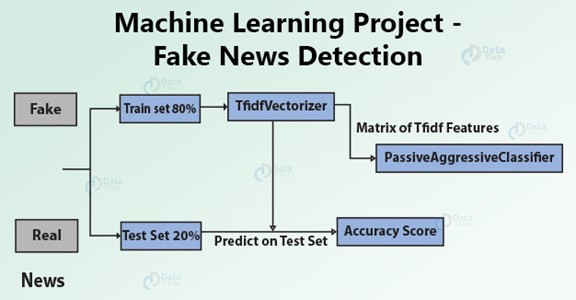
\includegraphics[width=8.8cm]{model.jpg}
    \caption{\underline{\textbf{Fig.}\ref{fig:project_view}}: Project Overview}
    \label{fig:project_view}
\end{center}

\subsection{Data collection and feature analysis}
\paragraph{Data Collection---}
Guardian newspaper and Kaggle provide an API( Application Program Interface) which enables to populate the model with up-to date news. These samples data are shared among 03 files under the names:   and .
\begin{itemize}
    \item \textit{'news.csv'} : which have a sample data of shape 6335 by 4 with 04 features ('Unnamed: 0', 'title', 'text', 'label') and contains a mixture of fake and real news.
    \item \textit{'Fake.csv'} : which have a sample data of shape 23481 by 4 with 04 features ('title', 'text', 'subject', 'date') and contains only fake news.
    \item \textit{'True.csv'} : which have a sample data of shape 21417 by 4 with 04 features ('title', 'text', 'subject', 'date') and contains only real news.
\end{itemize}

\paragraph{Feature Analysis---}
From the compiled samples data obtained above, we formed our experimental dataset based on 03 features which are \textit{'title', 'text', 'label'} with a shape of 51233 by 3 and contains a mixture of fake and real news.
\begin{itemize}
    \item \textbf{'title'} : The first column contains the title of the news.
    \item  \textbf{'text'} : The second column contains the plain-text news.
    \item \textbf{'label'} : The third column has labels denoting whether the news is REAL or FAKE.
\end{itemize}
\begin{center}
    \centering
    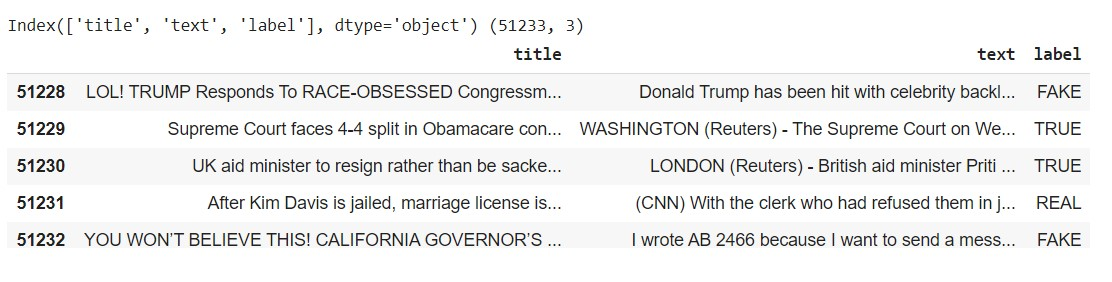
\includegraphics[width=8.8cm, height=4.4cm]{compiled dataset.jpg}
    \caption{\underline{Fig.\ref{fig:dataset}}: Compiled Dataset}
    \label{fig:dataset}
\end{center}
\underline{\textbf{NB:}} These samples data were taken from Guardian newspaper and Kaggle website where it can be found under the title \textit{Fake and Real news dataset}\cite{fakenewsdatasetkaggle}.
Kaggle provide an API(Application Program Interface) which enables to populate the dataset with up-to date news. The training and testing data were collected using the API.
\newline
\underline{\textbf{NB:}} This dataset is based on the topic of political news feeds in the USA and other countries with political instabilities.
\newline
In the next step, preprocessing of the dataset like removing stop words, punctuation marks, missing fields was done to sanitize the samples data.

\subsection{Description of the\\Classification Model}
\paragraph{Passive Aggressive algorithms}
are online learning algorithms. Such an algorithm remains passive for a correct classification outcome, and turns aggressive in the event of a miscalculation, updating and adjusting. Unlike most other algorithms, it does not converge. Its purpose is to make updates that correct the loss, causing very little change in the norm of the weight vector.

\subsubsection{Classification Model used}
For this research project, we decided to use a \textbf{Passive Aggressive Classification}(PAC) methodology as model.
\newline
Passive Aggressive Algorithms are a family of online learning algorithms (for both classification and regression) proposed by Crammer at al. \citep{crammer}.
The idea is very simple and their performance has been proofed to be superior to many other alternative methods.
\newline
The Passive-Aggressive algorithms are a family of Machine learning algorithms that are not very well known by beginners and even intermediate Machine Learning enthusiasts. However, they can be very useful and efficient for certain applications.\cite{geeksforgeeks}

\underline{\textbf{Note}}: This is a high-level overview of the algorithm explaining how it works and when to use it. It does not go deep into the mathematics of how it works.

\paragraph{Conceptual Understanding of PAC---}\cite{geeksforgeeks}
Passive-Aggressive algorithms are generally used for large-scale learning. In online machine learning algorithms, the input data comes in sequential order and the machine learning model is updated step-by-step, as opposed to batch learning, where the entire training dataset is used at once. This is very useful in situations where there is a huge amount of data and it is computationally infeasible to train the entire dataset because of the sheer size of the data. We can simply say that an online-learning algorithm will get a training example, update the classifier, and then throw away the example.
\newline
A very good example of this would be to detect fake news on a social media website like Twitter, where new data is being added every second. To dynamically read data from Twitter continuously, the data would be huge, and using an online-learning algorithm would be ideal.
\newline
Passive-Aggressive algorithms are somewhat similar to a Perceptron model, in the sense that they do not require a learning rate. However, they do include a regularization parameter.
\newline
\textbf{How Passive-Aggressive Algorithms Work:}\\
Passive-Aggressive algorithms are called so because :
\begin{itemize}
    \item \textbf{Passive}: If the prediction is correct, keep the model and do not make any changes. i.e., the data in the example is not enough to cause any changes in the model.
    \item \textbf{Aggressive}: If the prediction is incorrect, make changes to the model. i.e., some change to the model may correct it.
\end{itemize}

\paragraph{Mathematical Approach of PAC--- \citep{giuseppebonaccorso} \citep{crammer} \\}
Let’s suppose to have a dataset:
\begin{equation}
    \begin{cases} 
      X = \set{\overline{x}_0, \overline{x}_1, \dots, \overline{x}_t, \dots} where & \overline{x}_i \epsilon \mathbb{R}^n \\
      Y = \set{y_0, y_1, \dots, y_t, \dots} where & y_i \epsilon \set{-1, +1} \\
   \end{cases}
\end{equation}
The index t has been chosen to mark the temporal dimension. In this case, in fact, the samples can continue arriving for an indefinite time. Of course, if they are drawn from same data generating distribution, the algorithm will keep learning (probably without large parameter modifications), but if they are drawn from a completely different distribution, the weights will slowly forget the previous one and learn the new distribution. For simplicity, we also assume we’re working with a binary classification based on bipolar labels.
\newline
Given a weight vector w, the prediction is simply obtained as:
\begin{equation}
    \widetilde{y}_t = sign(\overline{w}^T * \overline{x}_t)
\end{equation}
All these algorithms are based on the Hinge loss function (the same used by SVM):
\begin{equation}
    L(\overline{\theta}) = \max(0, 1 - y * f(\overline{x}_i;\overline{\theta}))
\end{equation}
The value of $L$ is bounded between $0$ (meaning perfect match) and $K$ depending on $f(x(t),\theta)$ with $K>0$ (completely wrong prediction). A Passive-Aggressive algorithm works generically with this update rule:
\begin{equation}
    \begin{cases} 
      \overline{w}_{t+1} = \argmin_{\overline{w}} \frac{1}{2} \norm{\overline{w} - \overline{w}_t}^2 + C \xi^2\\
      L(\overline{w}; \overline{x}_t, y_t) \leq \xi \\
   \end{cases}
\end{equation}
To understand this rule, let’s assume the slack variable $\xi=0$ (and $L$ constrained to be $0$). If a sample $x(t)$ is presented, the classifier uses the current weight vector to determine the sign. If the sign is correct, the loss function is $0$ and the $\argmin$ is $w(t)$. This means that the algorithm is passive when a correct classification occurs. Let’s now assume that a misclassification occurred as show in figure \ref{fig:pac1}:
\begin{center}
    \centering
    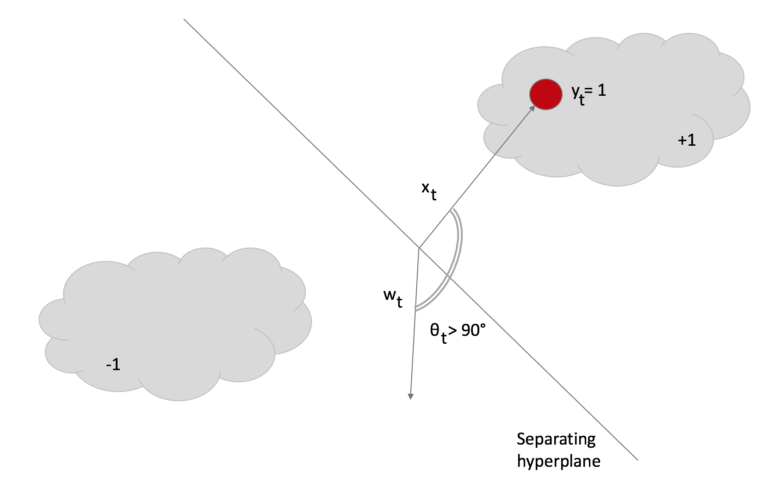
\includegraphics[width=8.8cm]{PAC1.png}
    \caption{\underline{\textbf{Fig.}\ref{fig:pac1}}}
    \label{fig:pac1}
\end{center}
The angle $\theta > 90\degree$, therefore, the dot product is negative and the sample is classified as $-1$, however, its label is $+1$. In this case, the update rule becomes very aggressive, because it looks for a new w which must be as close as possible as the previous (otherwise the existing knowledge is immediately lost), but it must satisfy $L=0$ (in other words, the classification must be correct).
\newline
The introduction of the slack variable allows to have soft-margins (like in SVM) and a degree of tolerance controlled by the parameter $C$. In particular, the loss function has to be $L \leq \xi$, allowing a larger error. Higher $C$ values yield stronger aggressiveness (with a consequent higher risk of destabilization in presence of noise), while lower values allow a better adaptation. In fact, this kind of algorithms, when working online, must cope with the presence of noisy samples (with wrong labels). A good robustness is necessary, otherwise, too rapid changes produce consequent higher misclassification rates.
\newline
After solving both update conditions, we get the closed-form update rule:
\begin{equation}
    \overline{w}_{t+1} = \overline{w}_t + \frac{\max(0, 1 - y_t(\overline{w}^T * \overline{x}_t))}{\norm{x_t}^2 + \frac{1}{2C}} y_t \overline{x}_t
\end{equation}
This rule confirms our expectations: the weight vector is updated with a factor whose sign is determined by $y(t)$ and whose magnitude is proportional to the error. Note that if there’s no misclassification the nominator becomes $0$, so $w(t+1) = w(t)$, while, in case of misclassification, w will rotate towards $x(t)$ and stops with a loss $L \leq \xi$. 
\newline
In the next figure \ref{fig:pac2}, the effect has been marked to show the rotation, however, it’s normally as smallest as possible:
\begin{center}
    \centering
    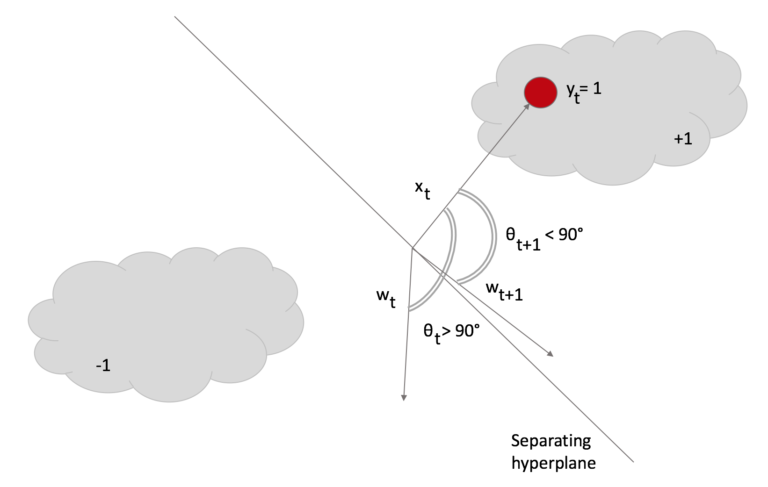
\includegraphics[width=8.8cm]{PAC2.png}
    \caption{\underline{\textbf{Fig.}\ref{fig:pac2}}}
    \label{fig:pac2}
\end{center}
After the rotation, $\theta < 90\degree$ and the dot product becomes negative, so the sample is correctly classified as $+1$.

\subsubsection{Architectural Diagram of the Classifier}
\begin{center}
    \centering
    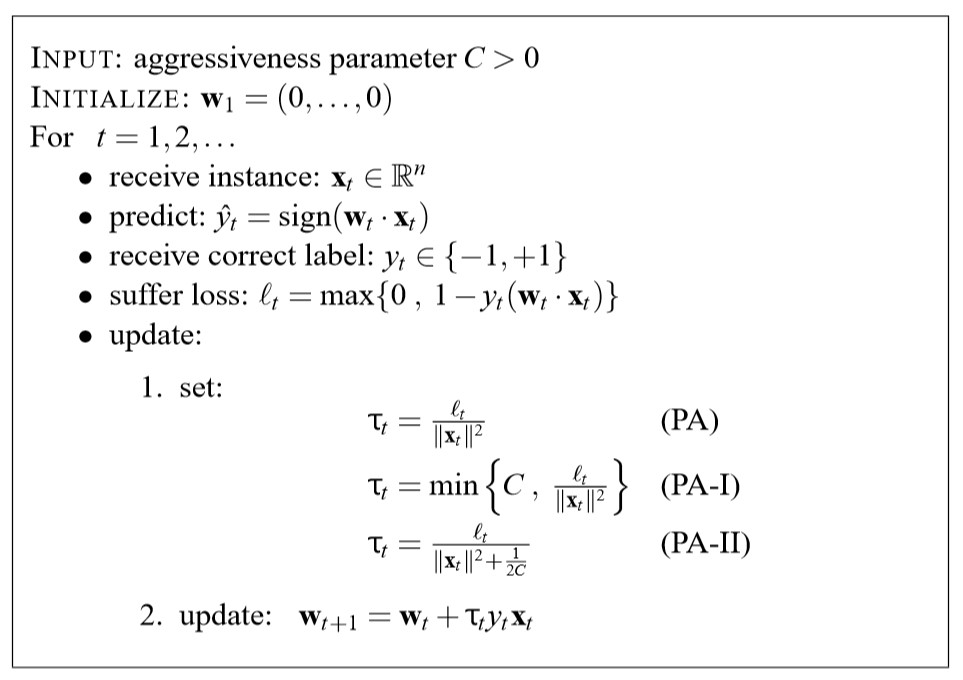
\includegraphics[width=8.8cm]{Three variants of the Passive-Aggressive algorithm for binary classification.jpg}
    \caption{\underline{\textbf{Fig.}\ref{fig:pac_var}}: Algorithm of Passive-Aggressive with its 03 variants(PA, PA-I, PA-II) used for binary classification.}
    \label{fig:pac_var}
\end{center}

\subsubsection{Explanation of the Parameters || Hyper-parameters}
\paragraph{}
Understanding the science behind this calculation isn't exceptionally basic and is past the extent of this research project. This research project gives only a diagram of the calculation and a basic usage of it.

\paragraph{Important parameters:}
\begin{itemize}
    \item \textbf{C} : This is the regularization parameter, and denotes the penalization the model will make on an incorrect prediction
    \item \textbf{max\_iter} : The maximum number of iterations the model makes over the training data.
    \item \textbf{tol} : The stopping criterion. If it is set to None, the model will stop when (loss $>$ previous\_loss  –  tol). By default, it is set to 1e-3.
\end{itemize}

\section{Implementation}
\paragraph{Fake News Detection ---}
is based on a Passive Aggressive Classification Algorithm. It was developed in Python using Google Colab Online IDE. The full implemented source code can be found under the GitHub Repository named \href{run: https://github.com/IUT-Thesis-Group-Cmr/ML-Project}{\textit{ML-Project}} \cite{projectgroup}

\subsection{Overview of the experiment}
\begin{center}
    \centering
    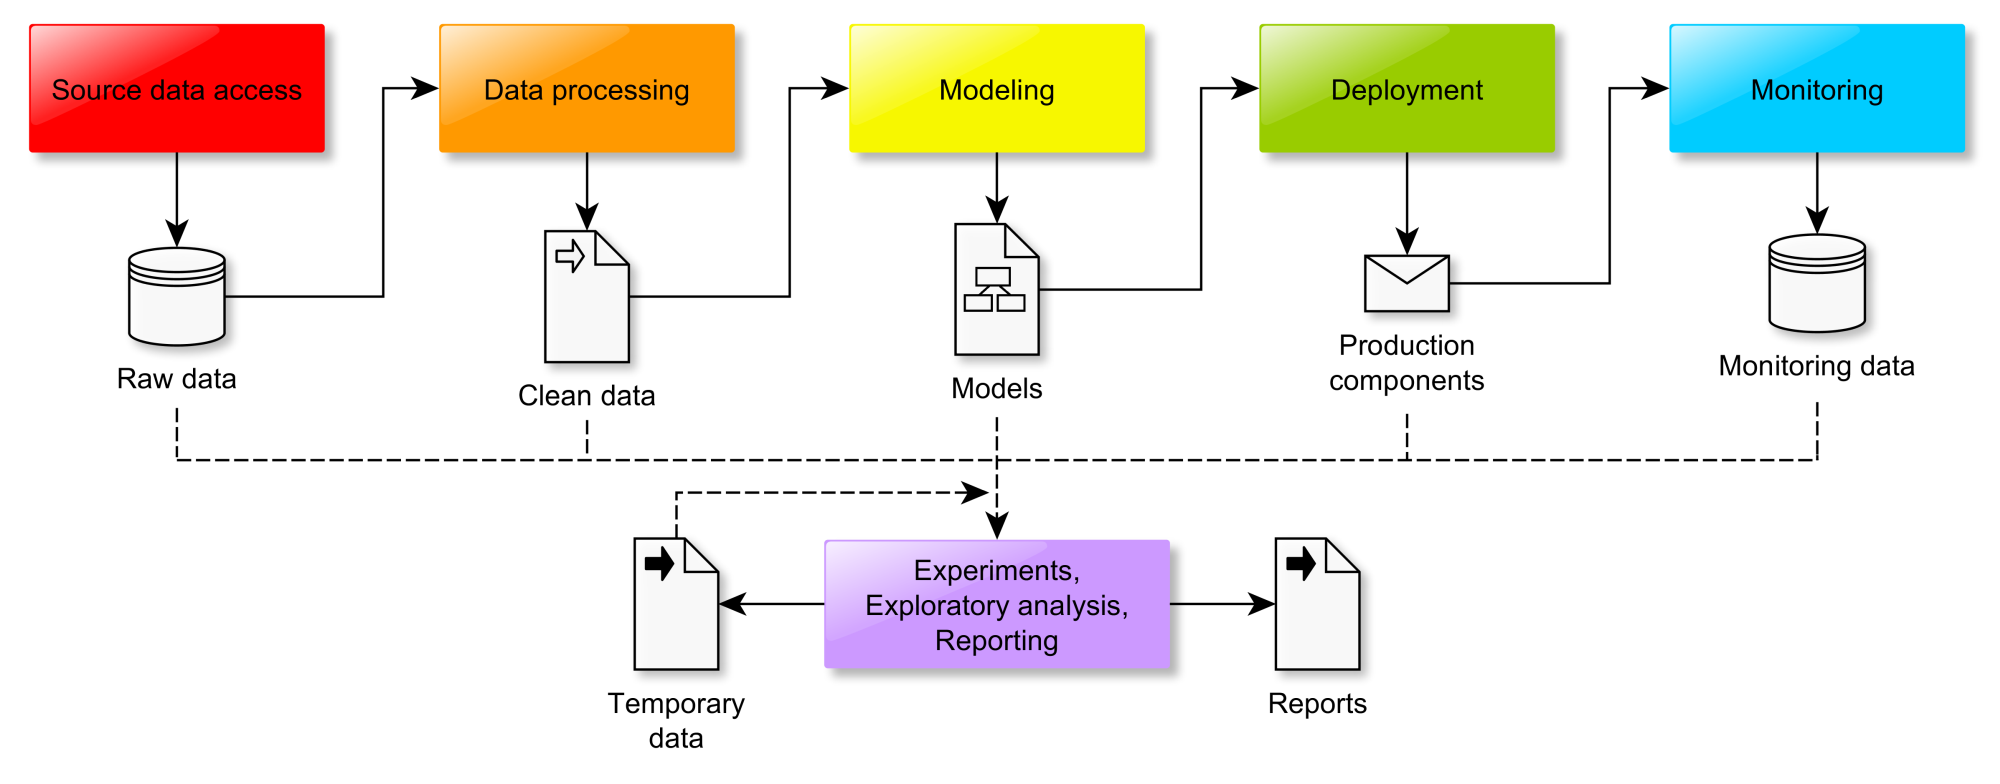
\includegraphics[width=8.8cm, height=5cm]{Data Science Workflow.png}
    \label{fig:framework}
\end{center}

\begin{center}
    \centering
    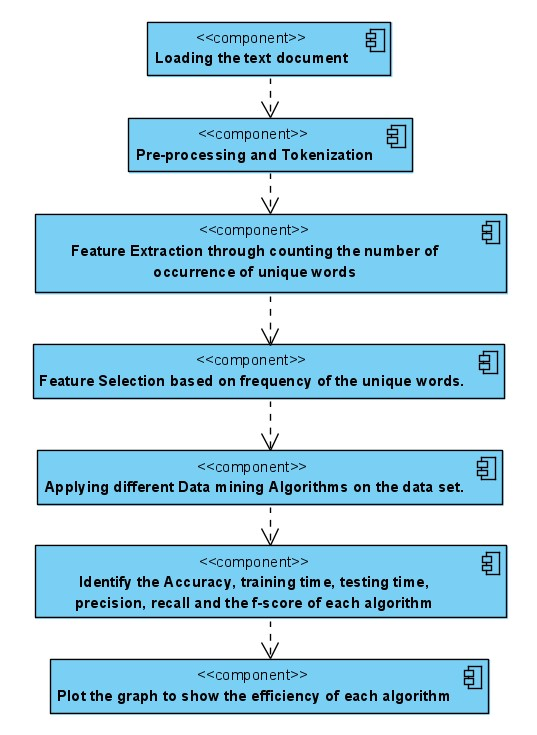
\includegraphics[width=8.8cm]{Workflow diagram of the framework proposed framework .jpg}
    \caption{\underline{\textbf{Fig.}\ref{fig:project_workflow}}: Workflow diagram of the framework proposed.}
    \label{fig:project_workflow}
\end{center}

\paragraph{Project Workflow Steps||}
\begin{itemize}
    \item Collecting Sample data related to Fake News Analysis.
    \item Building of a dataset from a set of known and well-done datasets.
    \item Loading and Analyzing dataset.
    \item Splitting the dataset into training and testing sets.
    \item Preprocessing of the dataset.
    \item Choose a Learning Model, Methodology or Schema for training the dataset.
    \item Fitting the Model with proper parameters and Predicting a feasible outcome(likelihood). 
    \item Determining the Model Accuracy Score.
    \item Report and Visualization of the predicted outcomes.
    \item If the results are not that convincing, then Tuning and Optimizing Model with necessary algorithms, is needed.
    \item Testing the Optimized Model, and Reporting its whereabouts and results.
    \item After Previous.Step, if the obtained results are not still that convincing then "Repeat Previous$\rightarrow$Previous.Step" with a more efficient technique.
    \item Summary Report on the Model.
\end{itemize}

\subsection{Feature engineering}
\paragraph{Feature engineering||}
is the process of using domain knowledge to extract features from raw data via data mining techniques. These features can be used to improve the performance of machine learning algorithms. Feature engineering can be considered as applied machine learning itself.
\paragraph{Feature Extraction||}
It uses data reduction which allows the elimination of less important features. The collection of words obtained through tokenization is sorted to find the unique words. The unique words and the count will be stored separately for further processing.\\
For this research project, we selected the features \textit{'text'} and \textit{'label'} from our compiled dataset shown in figure \ref{fig:selected_features} below.
\paragraph{Feature Selection||}
We used the feature \textit{'text'} as \textbf{input data} or data to be analyzed and the feature \textit{'label'} as \textbf{target data} or result/output from the input data.
\begin{center}
    \centering
    \qquad
    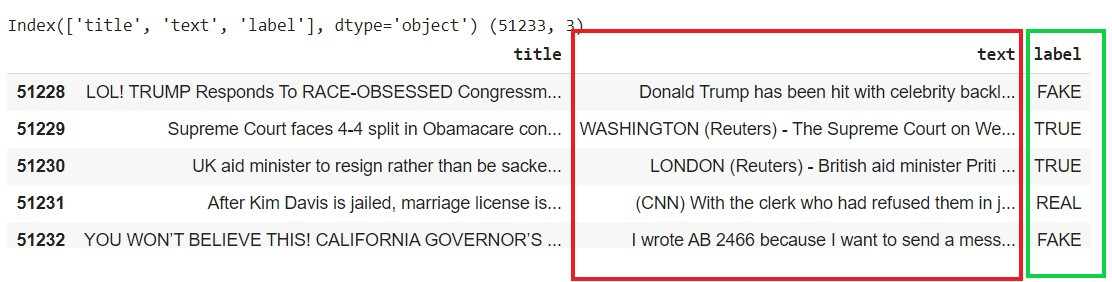
\includegraphics[width=8.8cm, height=3.9cm]{compiled dataset with selected features.jpg}
    \caption{\underline{Fig.\ref{fig:selected_features}}: Compiled Dataset with Selected features.}
    \label{fig:selected_features}
\end{center}
\paragraph{Data Preprocessing||}
To preprocess the data, we use a \textbf{TF-IDF Vectorizer} to transform the text to feature vectors that can be used as input to an estimator.\\
\newline
\underline{\textbf{What is a TF-IDF Vectorizer?}}\\
\textbf{TF-IDF} is an abbreviation for Term Frequency Inverse Document Frequency. This is very common algorithm to transform text into a meaningful representation of numbers which is used to fit machine algorithm for prediction. Let’s take sample example and explore two different spicy sparse matrix before go into deep explanation.
\begin{center}
    \centering
    \qquad
    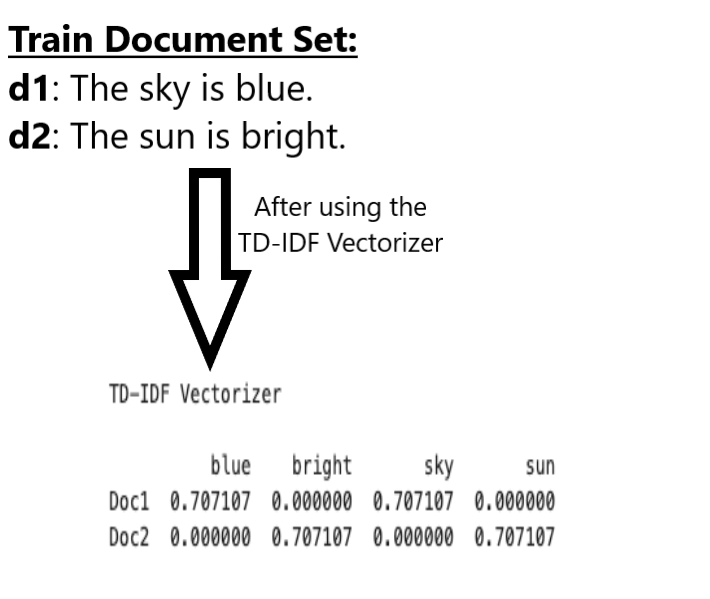
\includegraphics[width=8.8cm]{td-idf vect.png}
    \caption{\underline{Fig.\textbf{\ref{fig:td_idf_exple}}}: Text Document converted to Spicy Sparse Matrix of TF-IDF Vectorizer}
    \label{fig:td_idf_exple}
\end{center}
Here, we can see clearly that TF-IDF Vectorizer consider overall documents of weight of words. A vocabulary is a dictionary that converts each token (word) to a feature index in the matrix, each unique token gets a feature index.\\
The TF-IDF Vectorizer converts a collection of raw documents into a matrix of TF-IDF features.
\begin{itemize}
    \item \textbf{TF (Term Frequency)}: The number of times a word appears in a document is its Term Frequency. A higher value means a term appears more often than others, and so, the document is a good match when the term is part of the search terms.
    \item \textbf{IDF (Inverse Document Frequency)}: Words that occur many times a document, but also occur many times in many others, maybe irrelevant. IDF is a measure of how significant a term is in the entire corpus.
\end{itemize}\\
\newline
\textbf{Mathematical Understanding of TF-IDF||}\\
TF-IDF is a measure of originality  of a word by comparing the number of times a word appears in a document with the number of documents the word appears in.\\
\newline
\textbf{TF-IDF $= TF(t, d) * IDF(t)$}|| where $TF(t, d)$ is the number of times term $t$ appears in a document $d$ as shown:
\begin{equation}
    TF(t,d) = \sum_{x \epsilon d} fr(x,t)
\end{equation}
where $fr(x,t)$ is a simple function defined as:
\begin{equation}
    fr(x,t) = 
    \begin{cases} 
      1, & if \rightarrow x=t\\
      0, & otherwise\\
   \end{cases}
\end{equation}
and $\textbf{IDF}(t)$ is the Inverse Document Frequency which is computed as follow:
\begin{equation}
    IDF(t) = \log(\frac{1+n}{1+DF(d,t)}) +  1
\end{equation}
where $n$ is the number of documents and $\textbf{DF}(d,t)$ is the Document Frequency of the term $t$.
\paragraph{Remark||}
In \textbf{TfidfVectorizer} we consider \textbf{overall document weightage} of a word. It helps us in dealing with most frequent words. Using it we can penalize them. TfidfVectorizer weights the word counts by a measure of how often they appear in the documents.
\subsection{Training and Test Set Generation}
\paragraph{}
The train-test split procedure is used to estimate the performance of machine learning algorithms when they are used to make predictions on data not used to train the model.
\newline
It is a fast and easy procedure to perform, the results of which allow you to compare the performance of machine learning algorithms for your predictive modeling problem. Although simple to use and interpret, there are times when the procedure should not be used, such as when you have a small dataset and situations where additional configuration is required, such as when it is used for classification and the dataset is not balanced.\cite{traintestsplit}
\paragraph{Remark||}
The train-test split procedure is appropriate when you have a very large dataset, a costly model to train, or require a good estimate of model performance quickly.
\paragraph{}
In this research project, we used a split percentage of Train: 80\%, Test: 20\% which is also called a \textbf{8:2 split ratio} on the compiled dataset (figure \ref{fig:dataset}) with shape of 51233 by 3. We split the dataset with the selected features shown in figure \ref{fig:selected_features}.\\
After splitting the dataset, we got:
\begin{itemize}
    \item \textbf{X-Train}: with length $\{40986\}$ which represents 80\% of the dataset.
    \item \textbf{X-Test}: with length $\{10247\}$ which represents 20\% of the dataset.
    \item \textbf{Y-Train} and \textbf{Y-Test}: which are the target data for \textbf{X-Train} and \textbf{X-Test} respectively with the same split ratio.
\end{itemize}

\subsection{Running the Classifier}
\paragraph{Pre-Execution||}
Before executing the classifier, we use \textbf{TF-IDF Vectorizer} to sanitize, transform and preprocess both \textbf{X-Train} and \textbf{X-Test} as mentioned in the above sections. Thus, to obtain both \textbf{TF\_IDF-Train} and \textbf{TF\_IDF-Test} respectively (with more features) which are \textbf{vectorized versions} of X-Train and X-Test.
\paragraph{Execution||}
We use the obtained vectorized versions \textbf{TF\_IDF-Train} and \textbf{TF\_IDF-Test} to train and test the Passive Aggressive Classifier with their respective target samples.
While setting the PAC model, we configured some of its parameters with some values as shown below:
\begin{center}
    \centering
    \qquad
    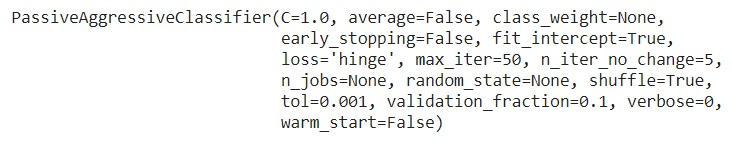
\includegraphics[width=8.8cm, height=3cm]{pac config.jpg}
    \label{fig:pac_config}
\end{center}

\section{Result Analysis}
\paragraph{}
To evaluate the performance of algorithms for fake news detection problem, various evaluation metrics have been used. In this subsection, we review the most widely used metrics for fake news detection. Most existing approaches consider the fake news problem as a classification problem that predicts whether a news article is fake or not:
\begin{itemize}
    \item True Positive (\textbf{TP}): when predicted fake news pieces are actually annotated as fake news;
    \item True Negative (\textbf{TN}): when predicted true news pieces are actually annotated as true news;
    \item False Negative (\textbf{FN}): when predicted true news pieces are actually annotated as fake news;
    \item False Positive (\textbf{FP}): when predicted fake news pieces are actually annotated as true news.
\end{itemize}
By formulating this as a classification problem, we can define following metrics,
\begin{equation}
    Precision = \frac{|TP|}{|TP|+|FP|}
\end{equation}
\begin{equation}
    Recall = \frac{|TP|}{|TP|+|FN|}
\end{equation}
\begin{equation}
    F1 = 2 * \frac{Precision * Recall}{Precision + Recall}
\end{equation}
\begin{equation}
    Accuracy = \frac{|TP| + |TN|}{|TP| + |TN| + |FP| + |FN|}
\end{equation}
\paragraph{}
These metrics are commonly used in the machine learning community and enable us to evaluate the performance of a classifier from different perspectives. Specifically, accuracy measures the similarity between predicted fake news and real fake news. Precision measures the fraction of all detected fake news that are annotated as fake news, addressing the important problem of identifying which news is fake. However, because fake news datasets are often skewed, a high precision can be easily achieved by making fewer positive predictions. Thus, recall is used to measure the sensitivity, or the fraction of annotated fake news articles that are predicted to be fake news. F1 is used to combine precision and recall, which can provide an overall prediction performance for fake news detection. Note that for Precision, Recall, F1, and Accuracy, the higher the value, the better the performance. 
\paragraph{}
The Receiver Operating Characteristics (\textbf{ROC}) curve provides a way of comparing the performance of classifiers by looking at the trade-off in the False Positive Rate (\textbf{FPR}) and the True Positive Rate (\textbf{TPR}). To draw the ROC curve, we plot the FPR on the x-axis and and TPR along the y-axis. The ROC curve compares the performance of different classifiers by changing class distributions via a threshold. $TPR$ and $FPR$ are defined as follows (note that TPR is the same as recall defined above):
\begin{equation}
    TPR = \frac{|TP|}{|TP|+|FN|}
\end{equation}
\begin{equation}
    FPR = \frac{|FP|}{|FP|+|TN|}
\end{equation}
Based on the ROC curve, we can compute the Area Under the Curve (AUC) value, which measures the overall performance of how likely the classifier is to rank the fake news higher than any true news. Based on \cite{roc}, AUC is defined as below.
\begin{equation}
    AUC = \frac{\sum (n_0 + n_1 + 1 + r_i) - n_0 (n_0 + 1)/2}{n_0 * n_1}
\end{equation}
where $r_i$ is the rank of $i^{th}$ fake news piece and $n_0 (n_1)$ is the number of fake (true) news pieces. It is worth mentioning that $AUC$ is more statistically consistent and more discriminating than accuracy \cite{stat_accuracy}, and it is usually applied in an imbalanced classification problem, such as fake news classification, where the number of ground truth fake news articles and and true news articles have a very imbalanced distribution.

\subsection{Overview}
\paragraph{}
In training, the model had an accuracy score of more than $97\%$. The model was able to predict whether an article was fake news 70\% of the time using the Fake News Net, Politifact and Kaggle dataset.
This dataset was chosen because it was formatted differently than the Fake News Net dataset. A benefit of the Politifact portion of the dataset is that it had an almost equal amount of real vs vake news samples, This ensured that the model was not biased towards real or fake in testing.

\subsection{Generation of Confusion-Matrix \& Heat-Map}
\paragraph{}
After training and testing the model, a confusion-matrix was generated and visualized as shown below:
\begin{equation}
    Confusion\_Matrix = 
    \begin{bmatrix}
        5168 & 125\\
        134 & 4820
    \end{bmatrix}
\end{equation}
\begin{center}
    \centering
    \qquad
    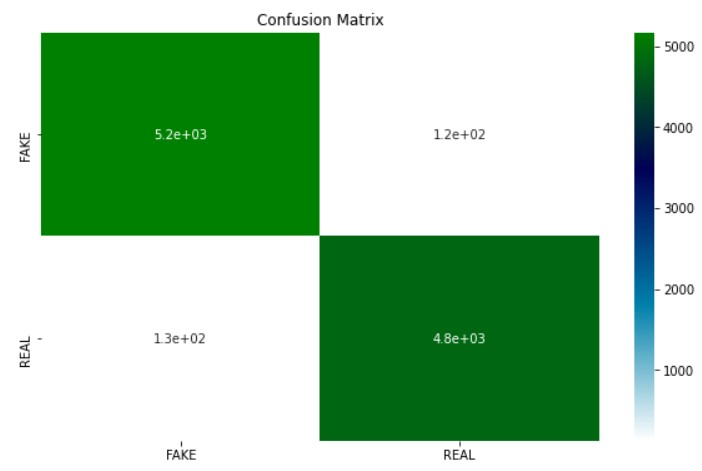
\includegraphics[width=8.8cm]{report4.jpg}
\end{center}

\subsection{Result analysis}
\begin{center}
    \centering
    \qquad
    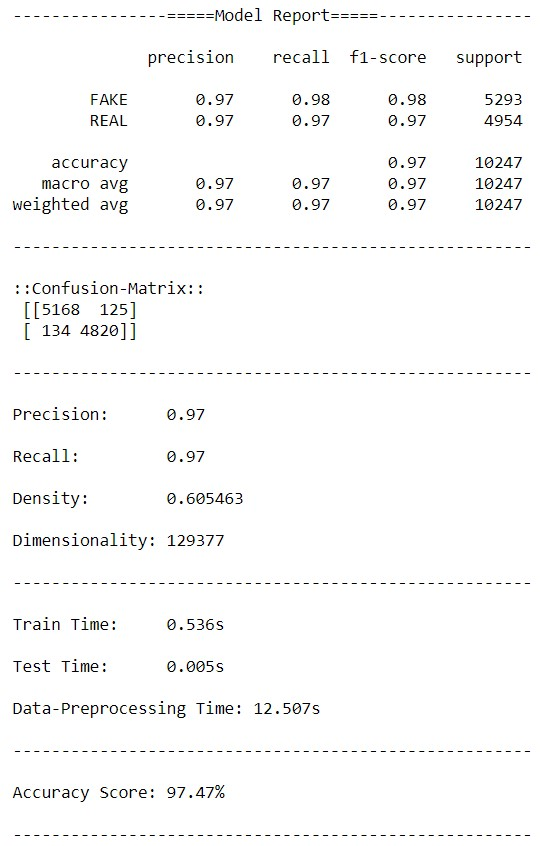
\includegraphics[width=8.8cm]{report1.jpg}
\end{center}

\begin{center}
    \centering
    \qquad
    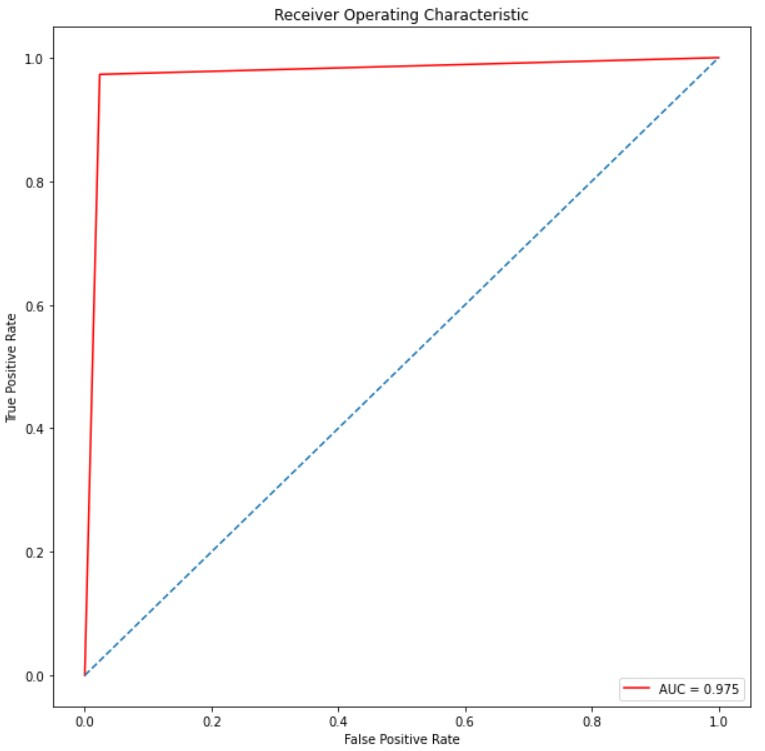
\includegraphics[width=8.8cm]{report2.jpg}
\end{center}
\begin{center}
    \centering
    \qquad
    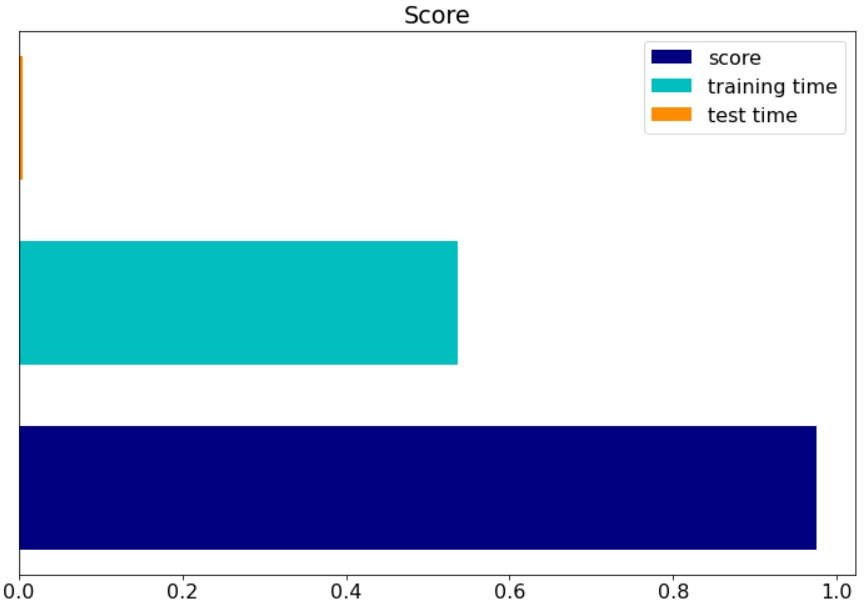
\includegraphics[width=8.8cm]{report5.jpg}
\end{center}

\begin{center}
    \centering
    \qquad
    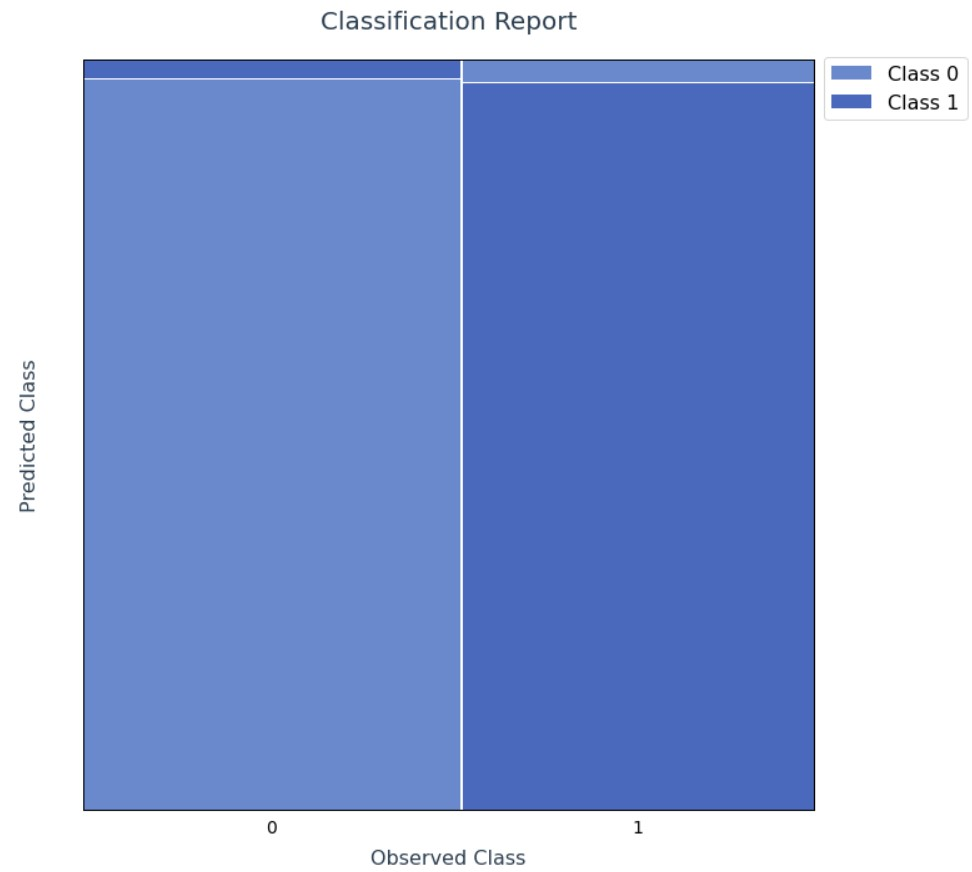
\includegraphics[width=8.8cm]{report6.jpg}
\end{center}

\section{Conclusion}
\paragraph{}
The problem of fake news has gained attention in 2016, especially in the aftermath of the last US presidential elections. Recent statistics and research show that $62\%$ of US adults get news on social media \cite{gottfried26}\cite{gottfried4}.\\
With the increasing popularity of social media, more and more people consume news from social media instead of traditional news media. However, social media has also been used to spread fake news, which has strong negative impacts on individual users and broader society.
\paragraph{}
It is certainly possible to classify news content into two types: fake news and real news, however there will always be an inherent bias to this classification based on the researcher’s own personal beliefs. Even though this is true, with tools like this research project it could be possible to at least cut down on the amount of objectively fake news that exists in the world today. With a preliminary result of 70\% this project could potentially contribute to accurately finding fake news and publicizing it, without the need for humans to have to do that work themselves.
\paragraph{}
The Efficiency can be improved using about five classifier models like Support Vector Machines, logistic Regression, Logistic Regression CV, which can perform better classification and can give a better accuracy. Using these classifiers, if the outputs are (REAL, REAL, FAKE, FAKE, REAL), then the output would be REAL as it is the majority. Apart from the classifier, we can also build a fact detector and a stance detector. Combination of all these tools would be the best  way to classify the news accurately.
\newline
Fake news detection is an emerging research area with few public datasets. We run our model on an existing dataset, showing that our model outperforms the original approach published by the authors of the dataset. 
\paragraph{}
In our future work, we will run our model on the few other publicly available datasets, such as the LIAR dataset which was released only recently, after we completed the current phase of our research.

\bibliographystyle{plain}
\bibliography{references}

\end{multicols}

\section*{\underline{Appendix A}: Code snippets}
In the new page, a snapshot of the entire source code of this research project can be found which is entitled \textit{\textbf{ML\_Project\_Fake\_News\_Detector}}. It contains a detail implementation of the proposed solution that tackles the stated problem illustrated in the above sections. It is written in iPython using Google Colab Online IDE and Jupyter Notebook IDE.
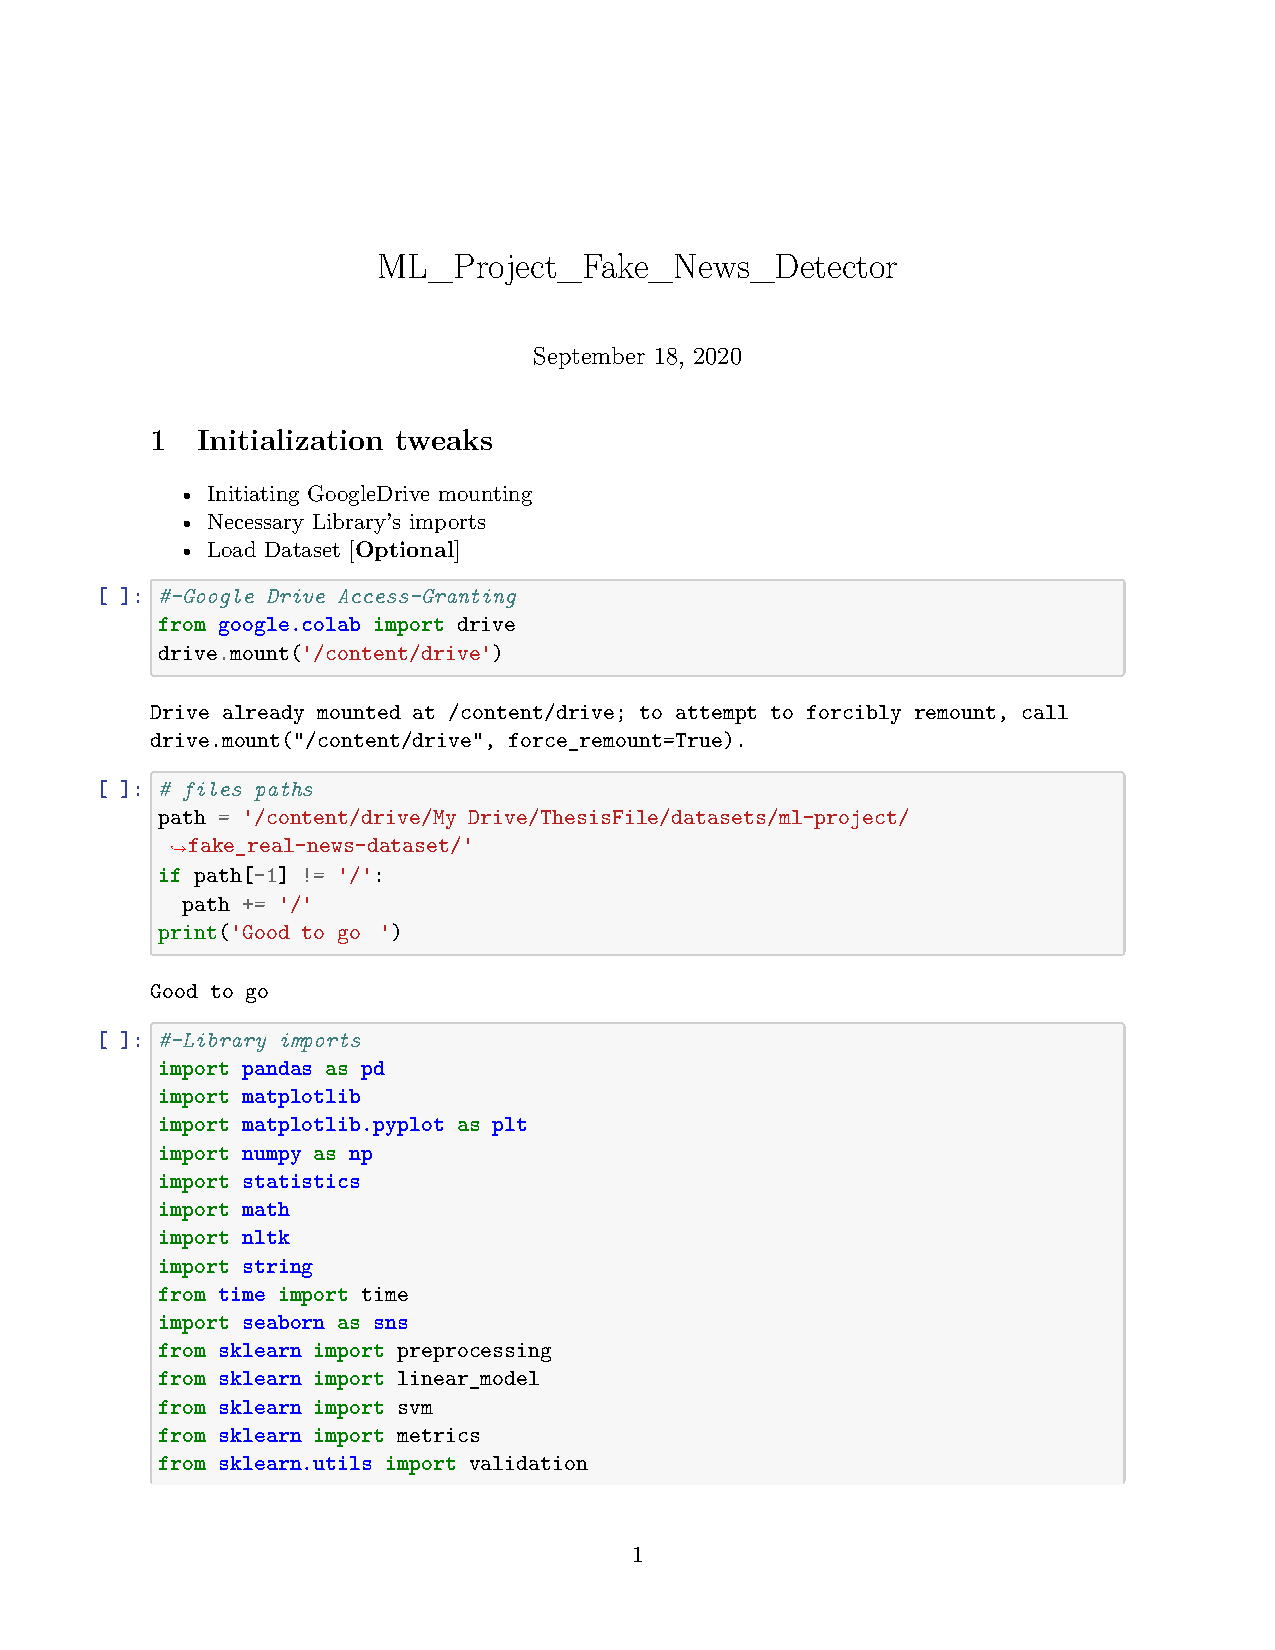
\includepdf[page=-]{ML_Project_Fake_News_Detector}

\end{document}
